\documentclass[12pt]{article}

\usepackage[margin=1in]{geometry} 
\usepackage{amsmath,amsthm,amssymb}
\usepackage{graphicx}

\newcommand{\N}{\mathbb{N}}
\newcommand{\Z}{\mathbb{Z}}

\newenvironment{exercise}[2][Exercise]{\begin{trivlist}
		\item[\hskip \labelsep {\bfseries #1}\hskip \labelsep {\bfseries #2.}]}{\end{trivlist}}

\makeatletter
\renewcommand*\env@matrix[1][*\c@MaxMatrixCols c]{%
	\hskip -\arraycolsep
	\let\@ifnextchar\new@ifnextchar
	\array{#1}}
\makeatother


\begin{document}
%\renewcommand{\qedsymbol}{\filledbox}

\title{Homework 4 (Due Sep 19, 2022)}%replace X with the appropriate number
\author{Jack Hyatt\\ %replace with your name
	MATH 574 - Discrete Mathamatics - Fall 2022} %if necessary, replace with your course title

\maketitle

\noindent

\medskip 

\begin{enumerate}


\item Give a double counting proof of the following: For all integers $n \geq 1$, 

\[\sum_{k=1}^n k {n \choose k} = n2^{n-1}.\]

The left side counts all possible ways to form a committee of any size from a group of $n$ people, with choosing someone in the committee to be the president of the committee.\medskip\\
The right side is choosing someone to be the president of a committee, then lining everyone else in the group up and choosing if they will be in the committee or not, which gets all possible committee of any size with a president.\qed

\medskip 

\item A 7-digit phone number (with digits in $0$-$9$) is selected randomly. What is the probability that the phone number has strictly increasing digits?\\\\
For the number of valid phone numbers, we consider the 10 digits 0-9 all lined up in a row. Then choose three of them to take out and we have a valid phone number. So the probability of a valid phone number will be $\frac{\binom{10}{3}}{10^7}$.

\medskip


\item Find the probability that a randomly generated bit string
of length $10$ does not contain a $0$ if bits are independent
and if
\begin{enumerate}
\item a $0$ bit and a $1$ bit are equally likely.\\\\
This is a 50/50 Bernoulli Trial for 10 successes in a row, which will be $\frac{1}{2}^{10}$.
\item the probability that a bit is a $1$ is $0.6$.\\\\
The same logic as before gives us $0.6^{10}$
\item the probability that the $i$th bit is a $1$ is $(\frac{1}{2})^i$ for $i =
1, 2, 3,\ldots, 10$.\\\\
It will be $(\frac{1}{2})^{1+\ldots+10} = (\frac{1}{2})^{55}$
\end{enumerate}

\medskip

\item A biased coin has probability for heads $3/4$ and tails $1/4$. A player flips the coin until a total of 3 tails show up. For $n \geq 1$, what is the probability that the player stops after $n$ flips?\\\\
This is very close to just 3 successes in $n$ Bernoulli Trials, but instead of the binomial coeff being normal, it will be choosing 2 spots for tails since the last flip will be the tail. So it is $\binom{n-1}{2}(\frac{1}{4})^3(\frac{3}{4})^{n-3}$. This also works for $n=1,2$ since the binomial coeff will equal 0, which makes sense.
\medskip

\item Find each of the following probabilities when $n$ independent Bernoulli trials are carried out with probability of success $p$. Note: $k$ successes in $n$ Bernoulli Trials is $\binom{n}{k}p^k(1-p)^{n-k}$
\begin{enumerate}
\item the probability of no failures\\\\
This is just clearly $p^n$.
\item the probability of at least one failure\\\\
This will be $1-p^n$
\item the probability of at most one failure\\\\
This is chance of 0 and 1 failure, $p^n + \binom{n}{1}p^{n-1}(1-p)^1$
\item the probability of at least two failures\\\\
This is 1 minus part (c), $1- (p^n + \binom{n}{1}p^{n-1}(1-p)^1)$.

\end{enumerate}


\medskip 


\item In the Erd\H{o}s--Renyi random graph model, a random graph $G(n,p)$ is generated as folllows: the vertex set of $G(n,p)$ is the set of $n$ vertices $\{1, 2, \ldots, n\}$. For each pair of distinct vertices $i$ and $j$, we add the edge $ij$ to the graph with probability $p$ (independently of the other edges). 

\begin{enumerate}
\item If $p > 0$, how large is the sample space of this experiment? That is, how many possible graphs $G(n,p)$ can be generated from this process?\\\\
The total number of edges in a complete graph is $\frac{n(n-1)}{2}$, and each edge has a choice of being in or not in (2 choices). So the total number of possible graphs will be $2^\frac{n(n-1)}{2}$

\item For a nonnegative integer $k$, what is the probability that the resulting graph $G(n,p)$ contains exactly $k$ edges?\\\\
This can be thought of as finding $k$ successes in $\frac{n(n-1)}{2}$ (number of possible edges) Bernoulli Trials. This formula is \[\binom{\frac{n(n-1)}{2}}{k}p^k(1-p)^{\frac{n(n-1)}{2}-k}\]

\item For a nonnegative integer $k$, what is the probability that a given vertex has exactly $k$ neighbors?\\\\
This can be thought of as finding $k$ successes in $n-1$ (number of possible neighbors) Bernoulli Trials. This formula is \[\binom{n-1}{k}p^k(1-p)^{n-1-k}\]

\end{enumerate}
\medskip

\item In a lottery, a set of 6 numbers are chosen randomly from $\{1, \ldots, 50\}$ (without repeats, and the order of the numbers do not matter). A person must pay \$1 to play the lottery. They select 6 numbers and win if and only if they get all 6 numbers correct.

\begin{enumerate}
\item Suppose the prize for winning is $1$ million dollars. What is the expected net profit for a player?\\\\
The probability of winning is $\frac{1}{\binom{50}{6}}$, so the expected value will be \[\frac{1}{\binom{50}{6}}(\$999,999)+ (1-\frac{1}{\binom{50}{6}})(-\$1)\]

\item Suppose that the prize of the lottery increases by $1$ million dollars at the end of every week if there is no winner. A player refuses to enter if their expected net profit is negative. How long must the player wait before they can play?\\\\
This can be solved by turning the above expression into a function of $x$ by replacing the \$999,999 with $1,000,000x+999,999$. Setting the function equal to 0 and solving for x results in just before 15, so the player must wait 15 weeks till they play.
\end{enumerate}

\medskip


\item You play a game of Plinko where a ball is placed at the top node and falls with gravity along the lines drawn. Each time the ball hits a peg (denoted by the nodes), the ball will either fall to the left or right with probability 1/2 each. In the end, the player wins a prize depending on which bin the ball lands in. See the image below.

\begin{center}
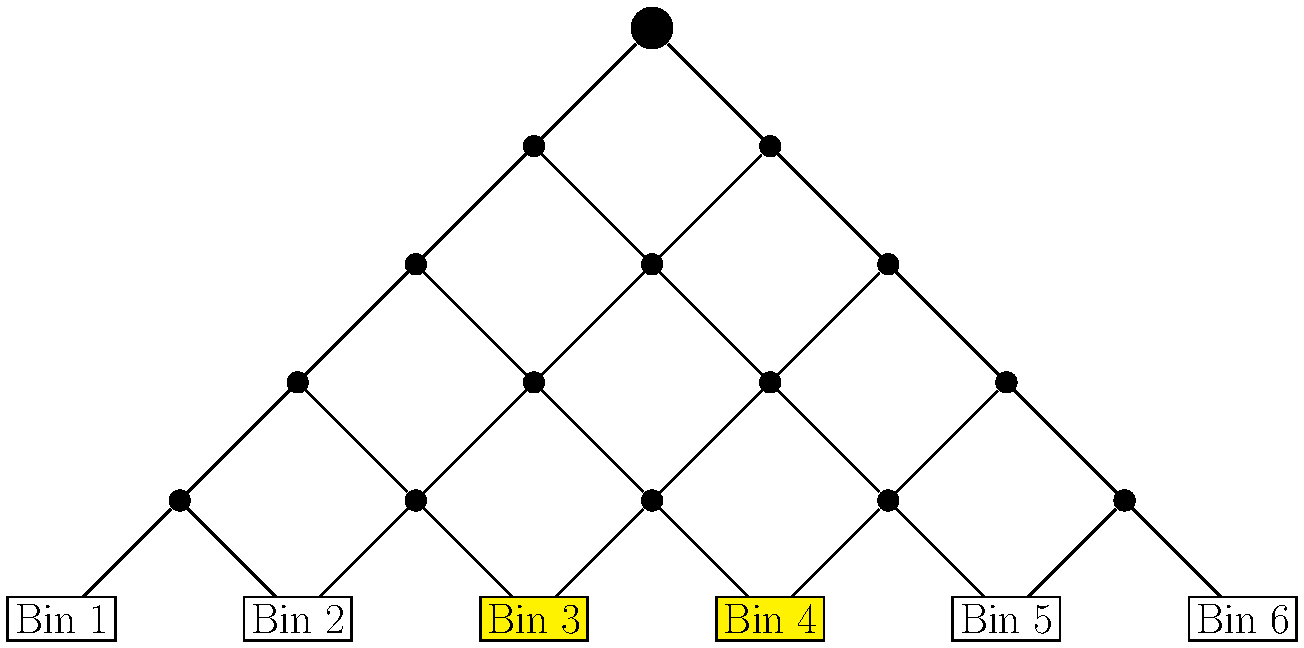
\includegraphics[scale=.66]{hw4_img1.pdf}
\end{center}

\begin{enumerate}
\item How many total paths are there from the top of the Plinko board to the bins?\\\\
At each layer, the ball will hit a node and fall either left or right. There are 5 layers, so the total number of paths will be $2^5$.

\item For $i = 1,2,3,4,5,6$, determine the probability that the ball lands in Bin $i$.\\\\
The total possible ways to get to $Bin_i$ is calculated by thinking that the ball needs to change directions $i-1$ times. Since there 5 layers for the ball to change directions, then the formula for paths to $Bin_i$ will be $\binom{5}{i-1}$. So the probability of landing in $Bin_i$ is $\frac{\binom{5}{i-1}}{2^5}$.

\item Suppose that the prize for landing in either Bin 1 or 6 is $\$5$ and the prize for landing in either Bin 2 or 5 is $\$1$. However if the ball lands in either Bin 3 or 4 then the player must pay $\$1$. What is the expected payout of the Plinko game?\\\\
Let $w_i$ be the amount won or lost for landing in $Bin_i$. The expected value will be \[\sum_{i=1}^{6} w_i\frac{\binom{5}{i-1}}{2^5} = 0\]
\end{enumerate}
\end{enumerate}
\end{document}
